\subsection{Volná rotace axiálně symetrického tělesa}
\label{sec:BodyRotation}
V prostoru volně rotuje axiálně symetrické těleso s momenty setrvačnosti $I$ vůči ose symetrie a $J$ vůči všem ostatním osám kolmým na osu symetrie a procházejícím těžištěm.
Natočení tělesa popsáno třemi Eulerovými úhly $(\phi,\theta,\psi)$,\index{úhly!Eulerovy}přičemž $\phi\in\langle0;2\pi)$ se nazývá \emph{precesní úhel} (popisuje otáční osy $Z$ spojené s tělesem vůči ose $z$ pevné v prostoru), $\theta\in\langle0;\pi)$ je \emph{nutační úhel} (popisuje úhel, který mezi sebou svírají osy $Z$ a $z$) a $\psi\in\langle0;2\pi)$ je \emph{rotační úhel} (popisuje natočení tělesa vůči ose $Z$), viz obrázek~\ref{fig:EulerAngles}\footnote{
	V praxi se souřadné systémy zavádějí tak, že osa $Z$ koinciduje s nějakým směrem významým v tělese, např. s osou symetrie, zatímco osa $z$ koinciduje se směrem významným v prostoru, např. se směrem magnetického pole.
}.
Vektor úhlové rychlosti rotace vzhledem k souřadnému systému spojenému s tělesem je
\begin{equation}
	\vector{\Omega}
		=\makematrix{0 \\ 0 \\ \dot{\psi}}
			+\underbrace{\matrix{R}_{3}(\psi)}
				_{\makematrix{\cos{\psi} & \sin{\psi} & 0 \\ -\sin{\psi} & \cos{\psi} & 0 \\ 0 & 0 & 1}}
				\makematrix{\dot{\theta} \\ 0 \\ 0}
			+\matrix{R}_{3}(\psi)\underbrace{\matrix{R}_{1}(\theta)}
				_{\makematrix{1 & 0 & 0 \\ 0 & \cos{\theta} & \sin{\theta} \\ 
					0 & -\sin{\theta} & \cos{\theta}}}
				\makematrix{0 \\ 0 \\ \dot{\phi}}\,,
\end{equation}
kde $\matrix{R}_{3}(\psi)$ přenese uzlovou přímku,\index{přímka!uzlová} která udává osu otáčení pro úhel $\theta$, na osu $X$, a $\matrix{R}_{1}(\theta)$ natočí osu $z$ podél uzlové přímky do směru osy $Z$.
Rozepsáním dostaneme \emph{Eulerovy kinematické rovnice}\index{rovnice!Eulerovy kinematické}
\begin{equation}
	\makematrix{\Omega_{1}\\ \Omega_{2}\\ \Omega_{3}}
		=\makematrix{\sin\theta\sin\psi & \cos\psi & 0 \\ \sin\theta\cos\psi & -\sin\psi & 0 \\
			\cos\theta & 0 & 1}\makematrix{\dot{\phi}\\ \dot{\theta}\\ \dot{\psi}}\,.
\end{equation}

\begin{figure}[!htbp]
	\centering
	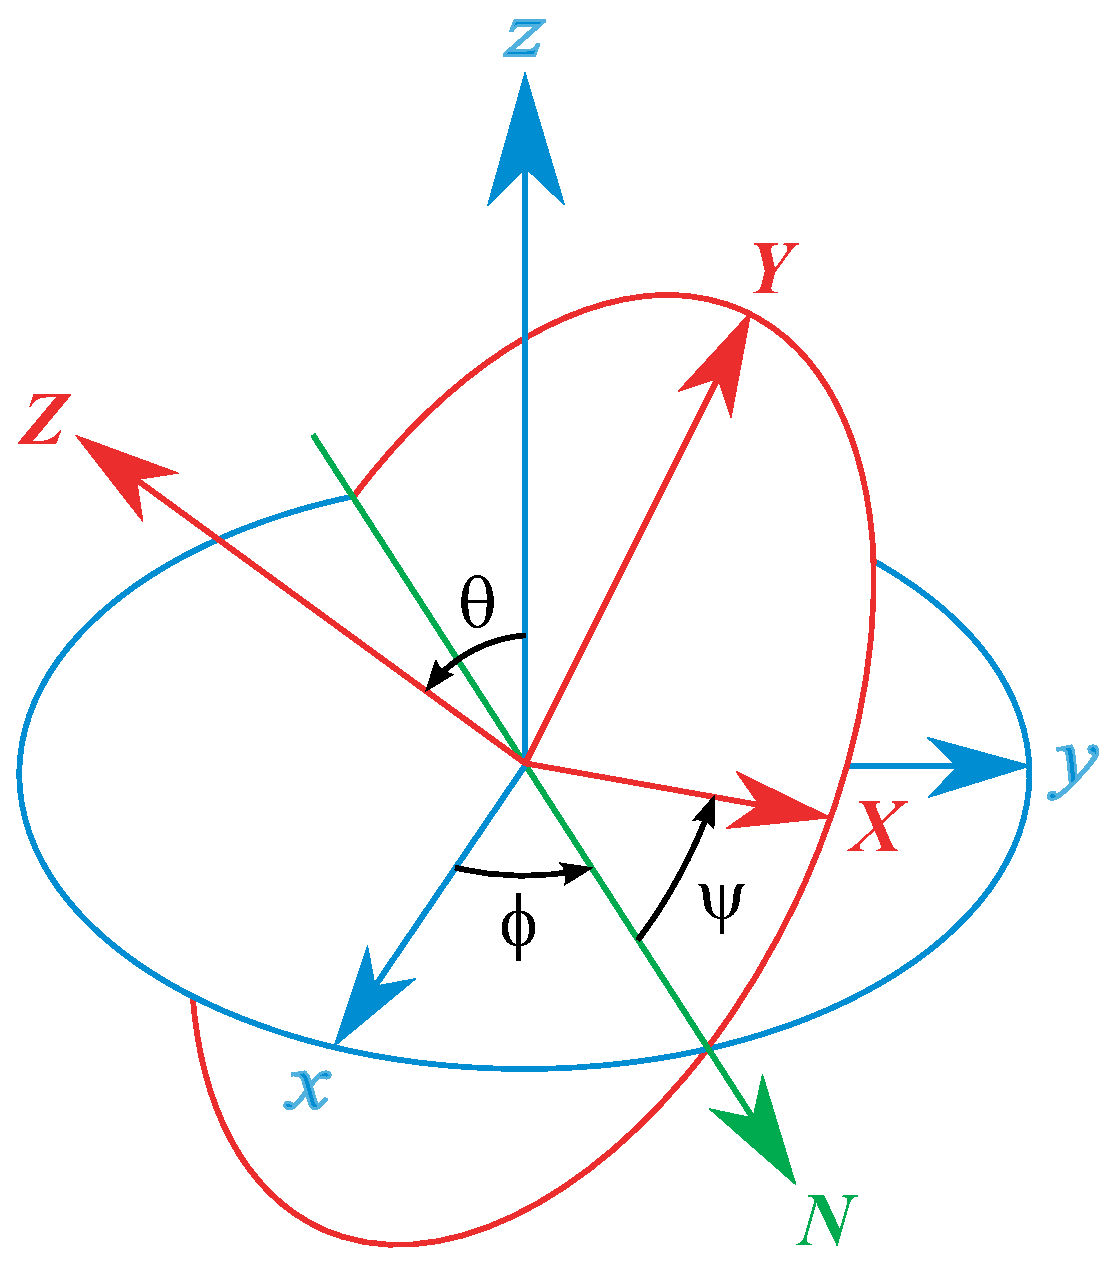
\epsfig{file=figures/euler.eps,width=0.4\linewidth}
	\caption{
		Eulerovy úhly. 
		Souřadná soustava $(x,y,z)$ pevná v prostoru (laboratorní soustava) je označena modře, souřadná soustava $(X,Y,Z)$ spojená s tělesem (těžišťová soustava) je označena červeně.
		Průsečnice rovin $(x,y)$ a $(X,Y)$, tzv. \emph{uzlová přímka}, je označena zeleně.
	}
	\label{fig:EulerAngles}
\end{figure}

\begin{enumerate}
\item 
	Napište Lagranžián za předpokladu, že osa symetrie tělesa je totožná s osou $Z$ 
	a počátek souřadné soustavy tělesa se nachází v jeho těžišti.

\item 
	Nalezněte metrický tenzor $\matrix{g}$, jeho determinant a 
	inverzní metrický tenzor $\matrix{g}^{-1}$.

\item 
	Určete Laplaceův operátor tohoto systému.

\item 
	Napište Schrödingerovu rovnici pro část závislou na úhlu $\theta$. 
	Využijte toho, že řešení Schrödingerovy rovnice lze separovat užitím substituce
	\begin{equation}
		\label{eq:BodyWaveFunction}
		u(\phi,\theta,\psi)=f(\theta)\e^{i(M\phi+K\psi)},
	\end{equation}
	kde $M$, $K$ jsou celá čísla.
\end{enumerate}
	
\begin{solution}
	\begin{enumerate}
	\item
		Pro pohyb volného tělesa je Lagranžián rovný kinetickému členu
		\begin{align}
			L&=\frac{1}{2}I\Omega_{3}^{2}
				+\frac{1}{2}J\left(\Omega_{1}^{2}+\Omega_{2}^{2}\right)\nonumber\\
			&=\frac{1}{2}I\left(\dot{\phi}\cos{\theta}+\dot{\psi}\right)^{2}
				+\frac{1}{2}J\left[\left(\dot{\phi}\sin{\theta}\sin{\psi}
				+\dot{\theta}\cos{\psi}\right)^{2}+\left(\dot{\phi}\sin{\theta}\cos{\psi}
				+\dot{\theta}\sin{\psi}\right)^{2}\right]\nonumber\\
			&=\frac{1}{2}I\left(\dot{\phi}\cos{\theta}+\dot{\psi}\right)^{2}
				+\frac{1}{2}J\left(\dot{\phi}^{2}\sin^{2}\theta+\dot{\theta}^{2}\right).
			\label{eq:BodyLagrangian}
		\end{align}
		
	\item
		V případě rotace tuhého tělesa, kdy zobecněné hmotnosti (momenty setrvačnosti) mohou být obecně v různých směrech různé, využijeme konvence~\eqref{eq:LagrangianHamiltonianCurvilinearM}.
		V našem případě je $(q^{1},q^{2},q^{3})=(\phi,\theta,\psi)$ a z~\eqref{eq:BodyLagrangian} plyne, že
		\begin{equation}
			\matrix{g}=\makematrix{I\cos^{2}\theta+J\sin^{2}\theta & 0 & I\cos{\theta} \\
						 0 & J & 0 \\
						 I\cos{\theta} & 0 & I}\,,
		\end{equation}
		\begin{equation}
			\det{g}
				=\left(I\cos^{2}\theta+J\sin^{2}\theta\right)JI-JI^{2}\cos^{2}\theta
				=IJ^{2}\sin^{2}\theta\,.
		\end{equation}
		K výpočtu inverzního metrického tenzoru využijeme vztahu
		\begin{equation}
			g^{kl}=(-1)^{k+l}\frac{\det{G_{ji}}}{\det g}\,,
		\end{equation}
		kde matici $G_{(ji)}$ získáme z matice $g$ vypuštěním $j$-tého řádku a $i$-tého sloupce.
		\begin{equation}
			\matrix{g}^{-1}
				=\makematrix{\frac{1}{J\sin^{2}\theta} & 0 & -\frac{\cos{\theta}}{J\sin^{2}\theta} \\
					0 & \frac{1}{J} & 0 \\
					-\frac{\cos{\theta}}{J\sin^{2}\theta} & 0 & 
						\frac{1}{I}+\frac{\cos^{2}\theta}{J\sin^{2}\theta}}\,.
		\end{equation}
		
	\item
		Laplaceův operátor je podle~\eqref{eq:Laplace}
		\begin{align}
			\Delta
				&=\frac{1}{J\sqrt{I}\sin{\theta}}\bigg\{\partialderivative{}{\phi}J\sqrt{I}\sin{\theta}
					\left(\frac{1}{J\sin^{2}\theta}\partialderivative{}{\phi}
					-\frac{\cos{\theta}}{J\sin^{2}\theta}\partialderivative{}{\psi}\right)\nonumber\\
				&\qquad+\partialderivative{}{\theta}J\sqrt{I}\sin{\theta}\frac{1}{J}\partialderivative{}{\theta}\nonumber\\
				&\qquad+\partialderivative{}{\psi}J\sqrt{I}\sin{\theta}
					\left[-\frac{\cos{\theta}}{J\sin^{2}\theta}\partialderivative{}{\phi}
					+\left(\frac{1}{I}+\frac{\cos^{2}\theta}{J\sin^{2}\theta}\right)
					\partialderivative{}{\psi}\right]\bigg\}\nonumber\\
				&=\frac{1}{J\sin^{2}\theta}\left[\partialderivative[2]{}{\phi}
					+\sin{\theta}\partialderivative{}{\theta}\sin{\theta}\partialderivative{}{\theta}
					-2\cos{\theta}\frac{\partial^{2}}{\partial\phi\partial\psi}
					+\left(\frac{J}{I}\sin^{2}\theta+\cos^{2}\theta\right)\partialderivative[2]{}{\psi}\right]\,.
				\label{eq:BodyLaplace}
		\end{align}
		
	\item
		Schödingerova rovnice pro vlnovou funkci~\eqref{eq:BodyWaveFunction} zní
		\begin{equation}
			-\frac{\hbar^{2}}{2}\Delta u(\phi,\theta,\psi)=Eu(\phi,\theta,\psi)\,,
		\end{equation}
		\begin{align}
			&\left[-M^{2}+\sin{\theta}\partialderivative{}{\theta}\sin{\theta}\partialderivative{}{\theta}+2MK\cos{\theta}
				-K^{2}\left(\frac{J}{I}\sin^{2}\theta+\cos^{2}\theta\right)\right]
				f(\theta)\e^{\im\left(M\phi+K\psi\right)}\nonumber\\
			&\qquad\qquad=-\frac{2J^{2}\sin^{2}\theta}{\hbar^{2}}Ef(\theta)
				\e^{\im\left(M\phi+K\psi\right)}
			\label{eq:BodySchrodinger}
		\end{align}

		Separace na část $f(\theta)$ a exponenciálu v úhlech $\phi$ a $\psi$ je možná, 
		jelikož Laplaceův operátor závisí na těchto úhlech jen přes derivace.
		Vlnová funkce musí dávat stejnou hodnotu po zvýšení $\phi$ a $\psi$ o úhel $2\pi$,
		\begin{subequations}
			\begin{align}
				u(\phi+2\pi,\theta,\psi)&=u(\phi,\theta,\psi),\\
				u(\phi,\theta,\psi+2\pi)&=u(\phi,\theta,\psi),
			\end{align}				
		\end{subequations}
		takže $M,K\in\mathbb{Z}$.
		Dá se nahlédnout, že tato vlastní čísla přísluší operátorům souvisejícím 
		s natočením okolo laboratorní osy $z$, respektive okolo osy spjaté s tělesem $Z$:
		\begin{subequations}
			\begin{align}
				\operator{M}u(\phi,\theta,\psi)&=-\im\partialderivative{}{\phi}u(\phi,\theta,\psi)=Mu(\phi,\theta,\psi)\,,\\
				\operator{K}u(\phi,\theta,\psi)&=-\im\partialderivative{}{\psi}u(\phi,\theta,\psi)=Ku(\phi,\theta,\psi)\,.
			\end{align}				
		\end{subequations}
		
		Rovnici~\eqref{eq:BodySchrodinger} převedeme na tvar
		\begin{equation}
			\label{eq:BodySchrodingerf}
			\derivative[2]{f}{\theta}+\frac{\cos{\theta}}{\sin{\theta}}\derivative{f}{\theta}
				-\frac{\left(M-K\cos{\theta}\right)^{2}}{\sin^{2}\theta}f+\sigma f=0\,,
		\end{equation}
		kde
		\begin{equation}
			\sigma=\frac{2EJ}{\hbar^{2}}-\frac{J}{I}K^{2}\,.
		\end{equation}
		V pokračování výpočtu postupujeme podle článku~\cite{Kronig1927}.
		Zavedeme substituce
		\begin{subequations}
			\begin{align}
				\lambda_{1}&=\frac{1}{2}\abs{K+M} & 
				\lambda_{2}&=\frac{1}{2}\abs{K-M} & 
				\lambda_{3}&=\frac{1}{2}+\sqrt{\frac{1}{4}+\sigma+K^{2}}\\
				\mu_{1}&=-\frac{1}{2}\abs{K+M} & 
				\mu_{2}&=-\frac{1}{2}\abs{K-M} & 
				\mu_{3}&=\frac{1}{2}-\sqrt{\frac{1}{4}+\sigma+K^{2}}
			\end{align}
			\begin{align}
				t&=\frac{1}{2}\left(\cos{\theta}+1\right)\nonumber\\
				F(t)&=\frac{f(t)}{t^{\lambda_{1}}(t-1)^{\lambda_{2}}}
			\end{align}				
		\end{subequations}
		a po dosazení do~\eqref{eq:BodySchrodingerf} dostaneme rovnici pro hypergeometrické funkce
		\begin{equation}
			t(1-t)\derivative[2]{F}{t}+\left[\gamma-(\alpha+\beta+1)t\right]\derivative{F}{t}-\alpha\beta F=0\,,
		\end{equation}
		kde
		\begin{subequations}
			\begin{align}
				\alpha&=\lambda_{1}+\lambda_{2}+\lambda_{3}\\
				\beta&=\lambda_{1}+\lambda_{2}+\mu_{3}\\
				\gamma&=2\lambda_{1}-1\,.
			\end{align}				
		\end{subequations}
		Řešení s dobrou asymptotikou dostaneme, pokud $\beta$ je nekladné celé číslo, 
		tj. $j=-\mu_{3}$ je nezáporné celé číslo.
		Dostáváme
		\begin{align}
			\left(j+\frac{1}{2}\right)^{2}&=\frac{1}{4}+\sigma+K^{2}\nonumber\\
			j(j+1)&=\sigma+K^{2}\nonumber\\
			\sigma&=j(j+1)-K^{2}\,,\nonumber
		\end{align}
		kde
		\begin{equation}
			j=(\lambda_{1}+\lambda_{2}),(\lambda_{1}+\lambda_{2}+1),\dotsc\,.
		\end{equation}
		Výsledné řešení včetně podmínek na kvantová čísla $j$, $K$, $M$ zní
		\begin{align}
			\label{eq:BodyEnergy}
			&\important{E_{jK}=\frac{\hbar^{2}}{2}\left[\frac{j(j+1)}{J}+K^{2}
				\left(\frac{1}{I}-\frac{1}{J}\right)\right]} &
			j&\in\mathbb{N}_{0}\,, & \abs{M}&\leq j\,, & \abs{K}&\leq j\,.
		\end{align}
	\end{enumerate}
				
	\begin{note}
		Spektrum volného axiálně symetrického tělesa bylo poprvé vyřešeno v práci~\cite{Kronig1927}.
	\end{note}
	
	\begin{note}
		Operátor celkového momentu hybnosti vůči soustavě spojené s tělesem 
		a jeho třetí komponenta jsou dány výrazy
		\begin{subequations}
			\begin{align}
				\operator{\mathcal{P}}^{2}
					&=-\frac{1}{\sin^{2}\theta}\left[\partialderivative[2]{}{\phi}
						+\sin{\theta}\partialderivative{}{\theta}\sin{\theta}\partialderivative{}{\theta}
						-2\cos{\theta}\frac{\partial^{2}}{\partial\phi\partial\psi}+\partialderivative[2]{}{\psi}\right]\\
				\operator{\mathcal{P}}_{3}
					&=-\im\partialderivative{}{\psi}.
			\end{align}				
		\end{subequations}
		Srovnáním s~\eqref{eq:BodyLaplace} dostaneme
		\begin{equation}
			\label{eq:tuheLaplaceP}
			\Delta=-\frac{\operator{\mathcal{P}}^{2}}{J}
				-\operator{\mathcal{P}}_{3}^{2}\left(\frac{1}{I}-\frac{1}{J}\right)
		\end{equation}
		a Schrödingerova rovnice má tvar
		\begin{equation}
			\label{eq:BodySchrodingerP}
			\frac{1}{2}\left[\frac{\operator{\mathcal{P}}^{2}}{J}
				-\operator{\mathcal{P}}_{3}^{2}\left(\frac{1}{I}-\frac{1}{J}\right)\right]
				u(\phi,\theta,\psi)=Eu(\phi,\theta,\psi)\,.
		\end{equation}
		Vlastní funkce operátoru $\operator{\mathcal{P}}^{2}$ jsou komplexně sdružené 
		Wignerovy $D$-funkce\index{funkce!Wignerovy $D$}\sfootnote{
			Wignerovy $D$-funkce ($D$-matice) jsou maticové elementy operátoru rotace
			\begin{equation}
				\operator{\mathcal{R}}(\phi,\theta,\psi)
					=\e^{-\im\psi\operator{J_{3}}}\e^{-\im\theta\operator{J_{2}}}\e^{-\im\phi\operator{J_{3}}}
			\end{equation}
			mezi vlastními stavy $\ket{jM}$ operátoru impulsmomentu a jeho třetí komponenty
			\begin{subequations}
				\begin{align}
					\operator{J}^{2}\ket{jM}&=j(j+1)\ket{jM}\\
					\operator{J}_{3}\ket{jM}&=M\ket{jM}
				\end{align}					
			\end{subequations}
			\begin{equation}
				D^{j}_{MK}(\phi,\theta,\psi)\equiv\matrixelement{jM}{\operator{\mathcal{R}}(\phi,\theta,\psi)}{jK}
					=\e^{-\im M\psi}d^{j}_{MK}(\theta)\e^{-\im K\phi}\,.
			\end{equation}
		}		
		\begin{equation}
			\operator{\mathcal{P}}^{2}D^{j*}_{MK}(\phi,\theta,\psi)
				=\hbar^{2}j(j+1)D^{j*}_{MK}(\phi,\theta,\psi)
		\end{equation}
		a působení $\operator{\mathcal{P}}_{3}$ na $D$-funkce je dáno výrazem
		\begin{equation}
			\operator{\mathcal{P}}_{3}D^{j*}_{MK}(\phi,\theta,\psi)=KD^{j*}_{MK}(\phi,\theta,\psi)\,.
		\end{equation}
		Po dosazení do~\eqref{eq:BodySchrodingerP} dostaneme spektrum~\eqref{eq:BodyEnergy} 
		a jako vlastní funkce komplexně sdružené Wignerovy $D$-funkce
		\begin{equation}
			u_{jMK}(\phi,\theta,\psi)=D^{j*}_{MK}(\phi,\theta,\psi)\,.
		\end{equation}
	\end{note}	

	\begin{note}
		Spektrum tuhého tělesa lze \uv{uhodnout} na pár řádcích.
		Hamiltonián tuhého tělesa se dá napsat jako
		\begin{align}
			\operator{H}
				&=\frac{1}{2J}\left(\operator{\mathcal{P}}_{x}^{2}+\operator{\mathcal{P}}_{y}^{2}\right)
					+\frac{1}{2I}\operator{\mathcal{P}}_{z}^{2}\nonumber\\
				&=\frac{1}{2J}\left(\vector{\operator{\mathcal{P}}}^{2}-\operator{\mathcal{P}}_{z}^{2}\right)
					+\frac{1}{2I}\operator{\mathcal{P}}_{z}^{2}\nonumber\\
				&=\frac{1}{2J}\vector{\operator{\mathcal{P}}}^{2}
					+\frac{1}{2}\left(\frac{1}{I}-\frac{1}{J}\right)\operator{\mathcal{P}}_{z}^{2},
		\end{align}
		kde $\vector{\operator{\mathcal{P}}}=\left(\operator{\mathcal{P}}_{x},\operator{\mathcal{P}}_{y},
		\operator{\mathcal{P}}_{z}\right)$ je operátor vektoru momentu hybnosti.
		Pokud předpokládáme, že jeho vlastní vektory jsou
		\begin{subequations}
			\begin{align}
				\vector{\operator{\mathcal{P}}}\ket{jK}&=\hbar^{2}j(j+1)\ket{jK}\,,\\
				\operator{\mathcal{P}}_{z}\ket{jK}&=\hbar K\ket{jK}\,,
			\end{align}				
		\end{subequations}
		dostaneme výraz~\eqref{eq:BodyEnergy}.	
	\end{note}
\end{solution}
